\documentclass[11pt]{article}

\usepackage[margin=1in]{geometry}
\usepackage[utf8]{inputenc}
\usepackage[T1]{fontenc}
\usepackage{amsmath,amssymb}
\usepackage{booktabs}
\usepackage{array}
\usepackage{graphicx}
\usepackage{xcolor}
\usepackage{enumitem}
\usepackage{caption}
\usepackage{float}
\usepackage[hidelinks,colorlinks=false]{hyperref}
\usepackage[noabbrev,capitalise]{cleveref}

\setlength{\parindent}{0pt}
\setlength{\parskip}{6pt}
\emergencystretch=3em

\definecolor{cIndigo}{HTML}{3A4CC4}
\definecolor{cAmber}{HTML}{96590A}
\definecolor{cInk2}{HTML}{525A6C}

\newcommand{\zv}{\mathbf{z}}

\title{\vspace{-2em}\textbf{Latent Horizon Geometry: Push-T}\\[0.3em]
\large How far the encoder moves, how far the predictor misses,\\
and where latent planning actually runs out of room}
\author{Companion to \texttt{latent-diagnostics-pusht.tex}; produced by
\texttt{scripts/latent\_horizon\_histograms.py}}
\date{8 September 2026}

\begin{document}
\maketitle
\vspace{-1.5em}

\begin{center}
\fcolorbox{cAmber}{white}{\parbox{0.95\textwidth}{\small
\textbf{Correction notice.} An earlier draft of this document reported predictor errors
roughly $6\times$ larger and concluded that LeWM's predictor was near-useless. That was a
measurement bug, not a property of the model: the actions were fed \emph{unnormalized}.
\Cref{sec:actionnorm} documents the bug, and \cref{sec:validation} validates the corrected
pipeline against the paper's own reported success rate. Every number below is post-fix.
The repo's pre-existing predictor diagnostics share the same bug and need re-running.}}
\end{center}

\section{What this measures}

Two distributions, at each prediction horizon $h$ measured in real environment steps.

\begin{enumerate}[leftmargin=1.4em,itemsep=2pt]
\item \textbf{True latent displacement} $\|\zv_t - \zv_{t+h}\|$. How far the frozen encoder
moves when the environment advances $h$ steps. This is the signal any latent distance has to
work with.
\item \textbf{Predictor error} $\|\zv_{t+h} - \widehat{\zv}(\zv_t, a_t \dots a_{t+h-1})\|$.
How far the autoregressive latent rollout lands from where the episode really went, given the
real actions the episode took.
\end{enumerate}

Neither is meaningful alone. Both are read against two reference scales measured on the same
data and checkpoint.

\textbf{The ceiling.} The median distance between two frames from \emph{different} episodes
is $\mathbf{19.76}$. Once a displacement reaches it, the encoder can no longer distinguish
"far" from "unrelated," so it is the saturation level.

\textbf{The no-motion baseline.} If the predictor returned $\zv_t$ unchanged, its error would
be \emph{exactly} the true displacement. So the ratio $\text{pred}/\text{disp}$ is the
fraction of the no-motion error that survives: $1.0$ means the rollout is worth nothing over
assuming the world froze, $0$ means perfect.

\section{The action-normalization bug}
\label{sec:actionnorm}

The model consumes \textbf{z-scored} actions, and this is easy to miss because nothing in
\texttt{jepa.py} says so. It is imposed by the data pipeline on both sides:

\begin{itemize}[leftmargin=1.4em,itemsep=2pt]
\item \textbf{Training:} \texttt{train.py} applies \texttt{utils.get\_column\_normalizer} to
every non-pixel column loaded, \texttt{action} included. That is a
\texttt{ZScoreNormalizer} built from the dataset's own mean and standard deviation.
\item \textbf{Evaluation:} \texttt{eval.py} fits a scikit-learn \texttt{StandardScaler} on
each cached column and hands it to \texttt{WorldModelPolicy} as \texttt{process}.
\end{itemize}

Push-T's action column has mean $\approx 0$ and standard deviation $\mathbf{0.206}$ per
dimension. Feeding raw actions therefore hands the predictor inputs about $\mathbf{4.9\times}$
too small, which the model reads as a near-stationary command. The result is a rollout that
behaves like a no-motion baseline, which is precisely the signature the earlier draft
reported.

\begin{table}[H]
\centering
\small
\caption{Median predictor error, before and after normalizing actions. Same checkpoint, same
samples, same rollout code.}
\begin{tabular}{rccc}
\toprule
$h$ & raw actions (wrong) & z-scored actions (correct) & true displacement \\
\midrule
5   & 4.04  & \textbf{1.00} & 5.14 \\
10  & 7.68  & \textbf{1.39} & 9.47 \\
25  & 15.22 & \textbf{2.42} & 16.89 \\
50  & 18.85 & \textbf{4.19} & 19.47 \\
80  & 19.28 & \textbf{6.30} & 19.62 \\
100 & 19.44 & \textbf{8.08} & 19.65 \\
\bottomrule
\end{tabular}
\end{table}

\textbf{This affects prior work in this repo.} \texttt{scripts/latent\_diagnostics.py}'s
\texttt{predictor\_error\_at\_block\_history} indexes the raw \texttt{action} column too, so
the recorded one-block ratio of $0.778$ on Push-T was computed under the same bug. The
corrected value is $\mathbf{0.195}$. Any conclusion resting on those diagnostics, including
the ratio and direction-agreement figures in \texttt{latent-diagnostics-pusht.tex}, should be
re-derived before being relied on.

Displacement and saturation measurements are \emph{unaffected}: they involve the encoder only
and never touch an action.

\section{Validation against the paper}
\label{sec:validation}

Since a measurement bug had already produced one confident wrong answer, the corrected
pipeline was checked against ground truth that does not depend on it: LeWM's own planning
evaluation.

\texttt{eval.py} was run with the pretrained \texttt{quentinll/lewm-pusht} checkpoint under
the paper's protocol, meaning goal $25$ steps ahead in the same trajectory, a $50$-step
budget, CEM with $300$ samples and $30$ iterations, horizon $5$ blocks, seed $42$, over $50$
trajectories.

\begin{table}[H]
\centering
\small
\caption{Push-T planning success rate.}
\begin{tabular}{lc}
\toprule
source & success rate (\%) \\
\midrule
Paper, Table 5 (mean $\pm$ std over 3 training seeds) & $96.0 \pm 2.83$ \\
This run, released checkpoint, 50 trajectories & $\mathbf{94.0}$ \\
\bottomrule
\end{tabular}
\end{table}

That is within one standard deviation of the reported value, so the checkpoint, the loader,
the preprocessing and the planner are all being driven correctly.

One patch was needed to get there and is worth recording. \texttt{swm.wm.utils.load\_pretrained}
fails outright on the released checkpoints, because they were saved by an older
\texttt{transformers} whose ViT block attributes have since been renamed. \texttt{eval.py} now
falls back to \texttt{scripts/common/lewm\_loader.py}, which carries the verified remap.

\section{Dataset: how long is an episode?}

\texttt{pusht\_expert\_train.h5} holds \textbf{18{,}685 episodes} and \textbf{2{,}336{,}736
frames}.

\begin{table}[H]
\centering
\small
\caption{Push-T episode length in environment steps, over all 18{,}685 episodes.}
\begin{tabular}{lcccccccccc}
\toprule
mean & median & std & min & max & p5 & p10 & p25 & p75 & p90 \\
\midrule
125.1 & 123 & 36.4 & 49 & 246 & 68 & 78 & 99 & 148 & 171 \\
\bottomrule
\end{tabular}
\end{table}

Measuring horizon $h$ needs an episode of at least $h+11$ steps, the $+11$ covering the
predictor's three-block history window. Every episode supports $h$ up to $25$; at $h{=}50$,
$98.4\%$ do; at $h{=}80$, $82.2\%$; at $h{=}100$, only $\mathbf{62.2\%}$, and those are by
construction the long episodes, meaning the ones the expert took longest to finish.

\begin{figure}[H]
\centering
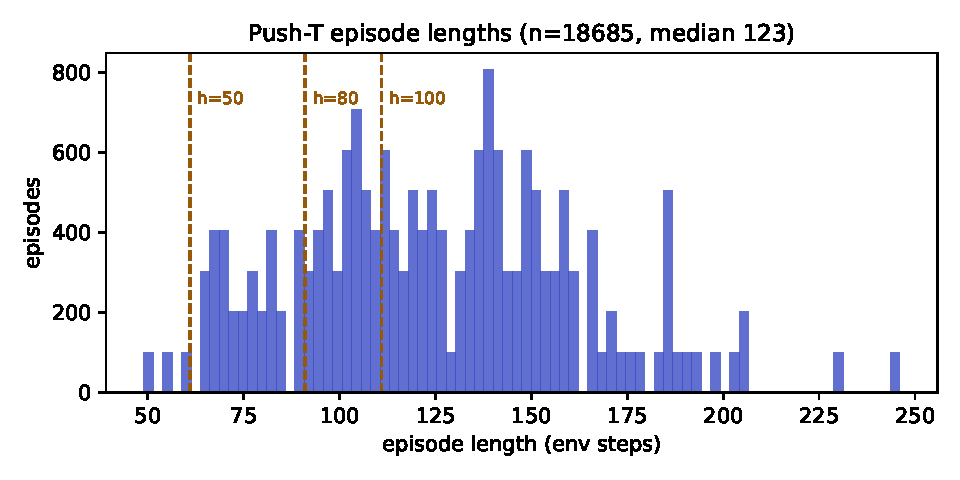
\includegraphics[width=0.68\textwidth]{figures/pusht_episode_lengths.pdf}
\caption{Episode lengths. Dashed lines mark the minimum length needed for $h{=}50$, $80$, $100$.}
\end{figure}

\section{Method}

800 episodes sampled uniformly at random, 99{,}021 frames, every frame encoded with the
pretrained checkpoint and episodes streamed one at a time so only embeddings are retained.
Displacements are taken over every valid $(t, t{+}h)$ pair, subsampled to at most 60{,}000 per
horizon. Rollouts follow the checkpoint's real convention: one predictor call spans
$\text{SKIP}{=}5$ environment steps and consumes a block of 5 concatenated 2-D actions, which
is exactly the \texttt{action\_encoder}'s 10 inputs; the rollout conditions on three history
blocks at $t{-}10$, $t{-}5$, $t$ and advances autoregressively for $h/5$ blocks, mirroring
\texttt{jepa.JEPA.rollout}. Actions are z-scored with the dataset's own statistics
(\cref{sec:actionnorm}). $h{=}1$ has no predictor arm, since a one-step forecast is not a
question this checkpoint was trained to answer.

\section{Results}

\begin{table}[H]
\centering
\small
\caption{Latent displacement and predictor error by horizon. Median with [q25, q75].
\emph{pred/disp} is the fraction of the no-motion error that survives; \emph{disp frac} is
the median displacement as a fraction of the $19.76$ ceiling.}
\begin{tabular}{rccccrr}
\toprule
$h$ & true displacement & predictor error & pred/disp & disp frac & $n_{\text{disp}}$ & $n_{\text{pred}}$ \\
\midrule
1   & 1.13\ \ [0.71, 1.64]   & ---                  & ---   & 0.06 & 60{,}000 & --- \\
5   & 5.14\ \ [3.42, 7.05]   & 1.00\ [0.82, 1.28]   & 0.195 & 0.26 & 60{,}000 & 60{,}000 \\
10  & 9.47\ \ [6.71, 12.12]  & 1.39\ [1.13, 1.82]   & 0.147 & 0.48 & 60{,}000 & 60{,}000 \\
25  & 16.89\ [13.81, 18.71]  & \textbf{2.42}\ [1.81, 3.48] & \textbf{0.143} & 0.85 & 60{,}000 & 60{,}000 \\
50  & 19.47\ [18.18, 20.31]  & 4.19\ [2.84, 6.54]   & 0.215 & 0.99 & 59{,}024 & 51{,}070 \\
80  & 19.62\ [18.66, 20.37]  & 6.30\ [4.11, 10.36]  & 0.321 & 0.99 & 35{,}938 & 29{,}054 \\
100 & 19.65\ [18.77, 20.38]  & 8.08\ [5.24, 13.41]  & 0.411 & 0.99 & 22{,}718 & 17{,}300 \\
\bottomrule
\end{tabular}
\end{table}

\begin{figure}[H]
\centering
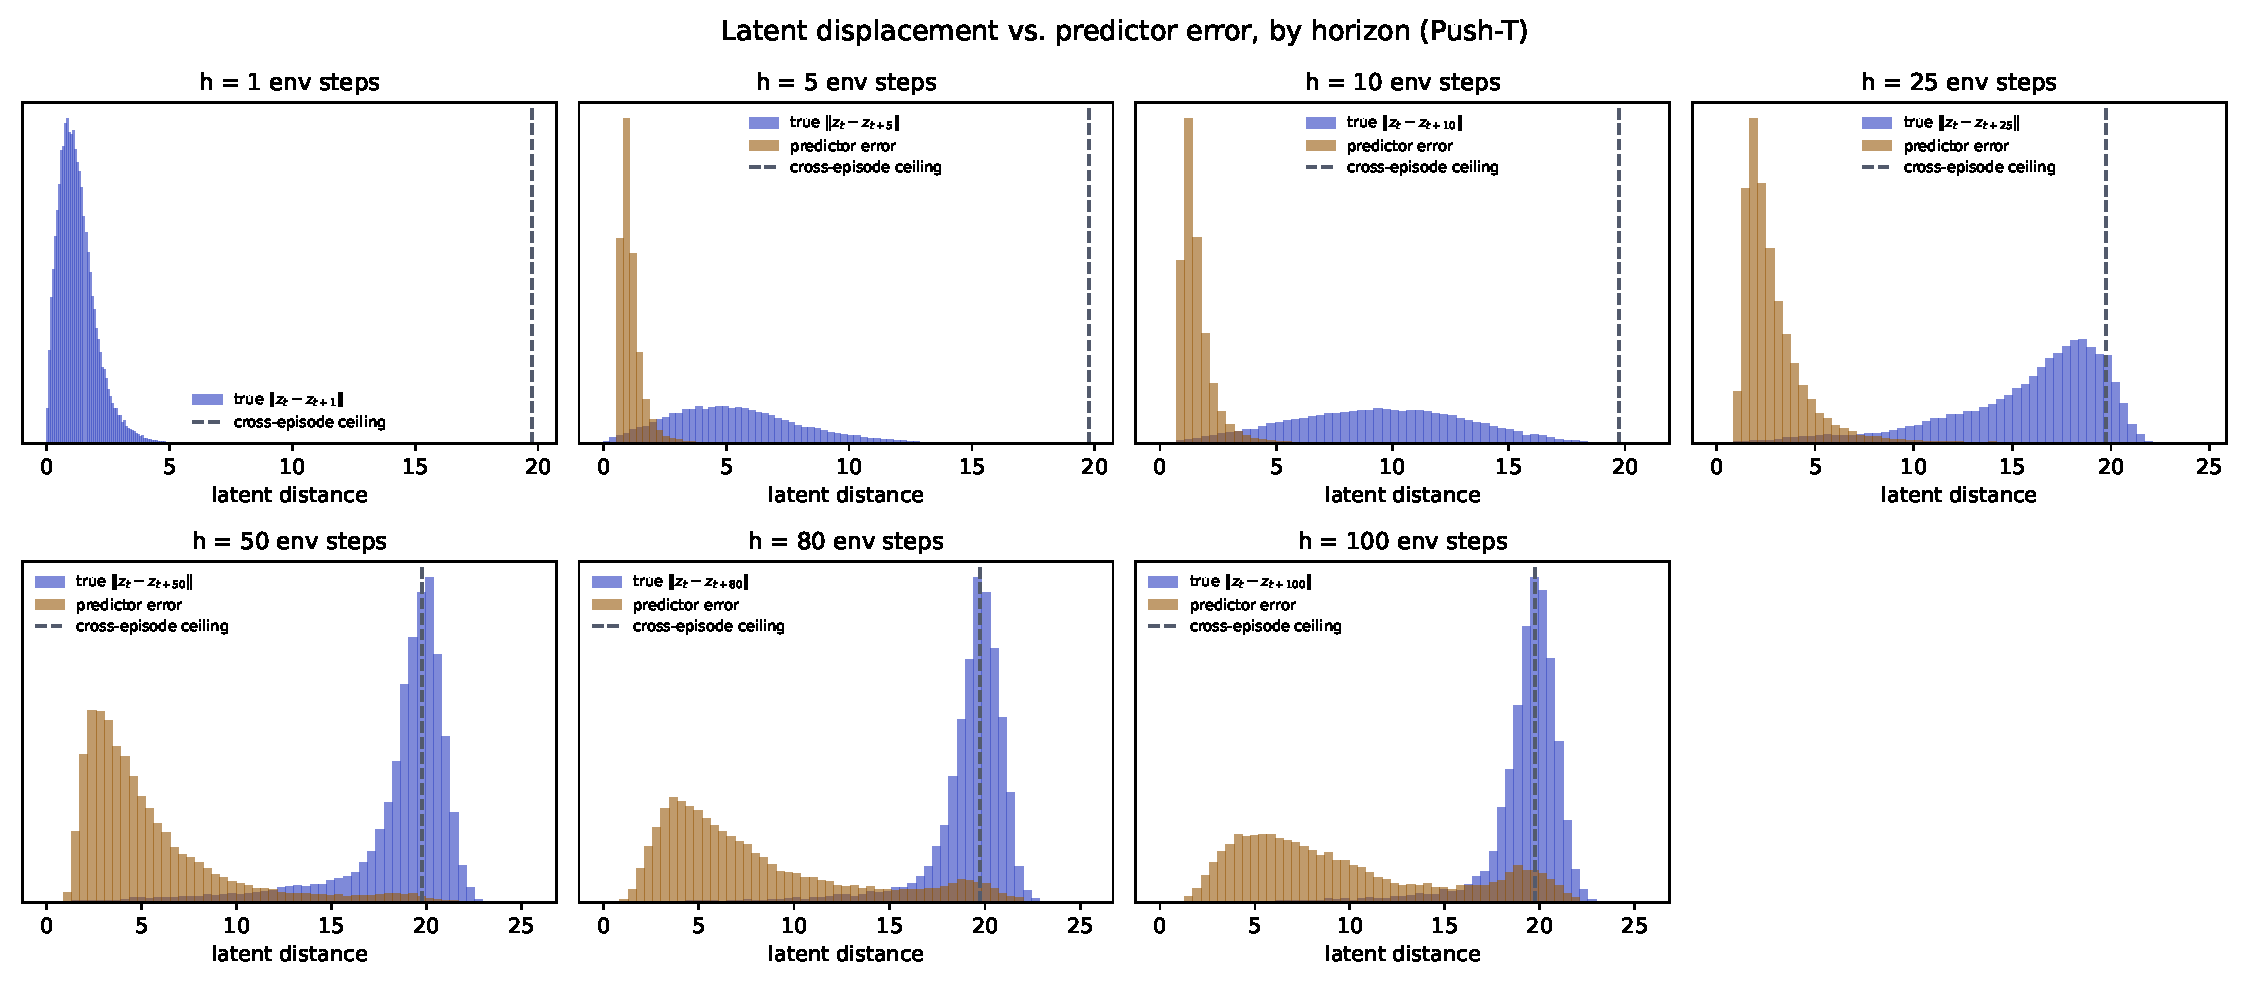
\includegraphics[width=\textwidth]{figures/pusht_horizon_histograms.pdf}
\caption{Per-horizon distributions. Blue is the true latent displacement, amber the predictor
error, dashed the cross-episode ceiling. The predictor error stays a small, well-separated
distribution well below the displacement it tracks, widening slowly with horizon.}
\end{figure}

\begin{figure}[H]
\centering
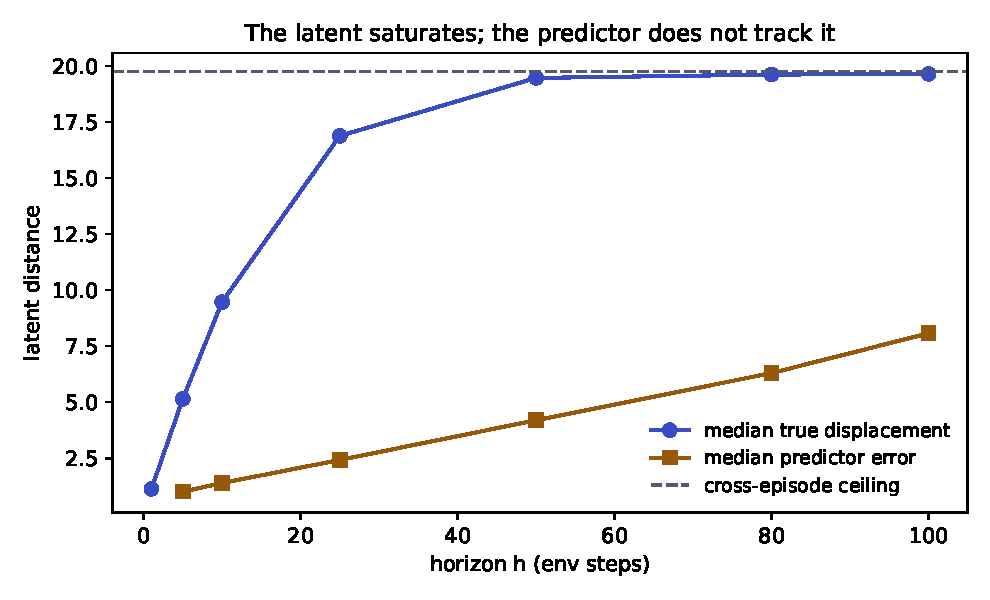
\includegraphics[width=0.72\textwidth]{figures/pusht_horizon_summary.pdf}
\caption{Medians against horizon. The displacement curve flattens against the ceiling by
$h{\approx}50$; the predictor error grows roughly linearly and stays far below it.}
\end{figure}

\section{Findings}

\textbf{1. The predictor is accurate, and most accurate exactly where LeWM plans.} At
$h{=}25$, the planner's own horizon, the rollout's median error is $2.42$ against a
displacement of $16.89$. It removes about $86\%$ of the no-motion error. Even after twenty
autoregressive blocks at $h{=}100$ the error is $8.08$, still well under the $19.76$ ceiling.
The predictor is doing real work at every horizon tested.

\textbf{2. The encoder saturates at about 50 environment steps.} Median displacement reaches
$85\%$ of the ceiling by $h{=}25$ and $98.5\%$ by $h{=}50$. Past that, two frames from the
same episode are as far apart as two frames from unrelated episodes. This measurement involves
no actions and was unaffected by the bug.

\textbf{3. The binding constraint on latent planning is the encoder's range, not the
predictor.} This is the corrected version of the earlier claim, and it reverses its direction.
Past $h \approx 50$ the distance cannot discriminate between candidates \emph{even given a
perfect prediction}, because every separation reads as maximal. Before that point the
predictor is accurate enough that the planner works, which is what the $94\%$ success rate in
\cref{sec:validation} demonstrates.

The complementary measurement, from \texttt{scripts/planning\_cost\_gate.py} under the same
fix, agrees. Ranking $24$ candidate action sequences against what the simulator actually does,
over $100$ planning problems:

\begin{table}[H]
\centering
\small
\caption{Spearman of each cost against the true outcome, and normalized regret (0 = the cost
picks the genuinely best candidate, 1 = the worst). \emph{deployed} scores the predictor's
guess; \emph{true state} applies the same cost to the state actually reached.}
\begin{tabular}{rcccc}
\toprule
goal offset & deployed $\rho$ & true-state $\rho$ & deployed regret & true-state regret \\
\midrule
25  & \textbf{0.839} & 0.888 & \textbf{0.021} & 0.006 \\
50  & 0.519 & 0.580 & 0.168 & 0.147 \\
100 & 0.270 & 0.283 & 0.307 & 0.314 \\
\bottomrule
\end{tabular}
\end{table}

At the paper's operating point the deployed cost nearly matches what is achievable with
perfect prediction, and picks essentially the best candidate available. The two columns then
fall together as the goal moves out, which is the saturation of finding 2, not a failure of
the predictor.

\section{Caveats}

\begin{enumerate}[leftmargin=1.4em,itemsep=3pt]
\item \textbf{Rollouts are fed the real actions.} A planner feeds hypothetical candidates,
which are off-distribution. These are a best case for the predictor.
\item \textbf{The two long horizons are conditioned on long episodes.} $h{=}80$ and $h{=}100$
exist in only $82\%$ and $62\%$ of episodes, and those are the slowest ones. Saturation is
already established at $h{=}50$ across $98.4\%$ of the dataset, so the conclusion is
unaffected, but those two rows are not unconditional dataset statistics.
\item \textbf{One environment, one checkpoint.} Two-Room's ratio of one-step movement to
overall latent spread is far less extreme, so it should saturate substantially later. Running
it is a single flag change.
\item \textbf{Medians, not means.} All distributions are right-skewed; quartiles are in the
table for that reason.
\end{enumerate}

\section{Reproducing}

\begin{verbatim}
# horizon histograms
python scripts/latent_horizon_histograms.py --env pusht \
    --n-episodes 800 --max-samples 60000 --out outputs/latent_horizon_pusht

# candidate-ranking gate
python scripts/planning_cost_gate.py --env pusht --n-problems 100 \
    --n-candidates 24 --goal-offsets 25 50 100

# the paper's own planning eval (STABLEWM_HOME must hold datasets/ and checkpoints/)
python eval.py policy=lewm-pusht eval.num_eval=50
\end{verbatim}

\end{document}
